% Section 3 (structure-learning part). Draft by Zachary; numbers are from structure_learning.ipynb (PYTHONHASHSEED=0).
% Requires \usepackage{booktabs, graphicx, amsmath}. Upload figures/structure/report_dags.png and
% models/structure_table.tex to the same relative paths in Overleaf, or adjust the paths below.

\subsection{Network structure}

\paragraph{Hand-designed DAG.}
From domain intuition we drew the DAG in Fig.~\ref{fig:dags}a. Following our proposal, popularity has three parents (energy, danceability and decade), which caps its CPT at $4 \times 5^3 = 500$ free parameters. Loudness was dropped in preprocessing as nearly redundant with energy.

\paragraph{Structure learning.}
We ran Hill Climb (HC) search on the training set, scored with
$\mathrm{BIC}(G) = \log P(\mathcal{D} \mid \hat\theta_G, G) - \tfrac{\log N}{2}\dim(G)$,
which charges about $4.1$ nats per free parameter. To cover multiple configurations, we also varied:
\begin{itemize}
  \item the HC setup: in-degree caps, popularity forced to be a sink, and a warm start from the hand DAG;
  \item the score: AIC, K2, and BDeu with ESS $\in \{1, 10, 100\}$;
  \item the algorithm: GES, PC, Chow-Liu, Naive Bayes and TAN;
  \item popularity's parent set, searched exhaustively for each size $k \le 4$.
\end{itemize}
HC optimizes BIC directly, so we also chose between structures by 5-fold cross-validated (CV) log-loss of $P(\text{popularity} \mid \text{all other variables})$, rerunning the search inside each fold. We also measured edge stability over 200 bootstrap resamples.

\begin{figure}[t]
  \centering
  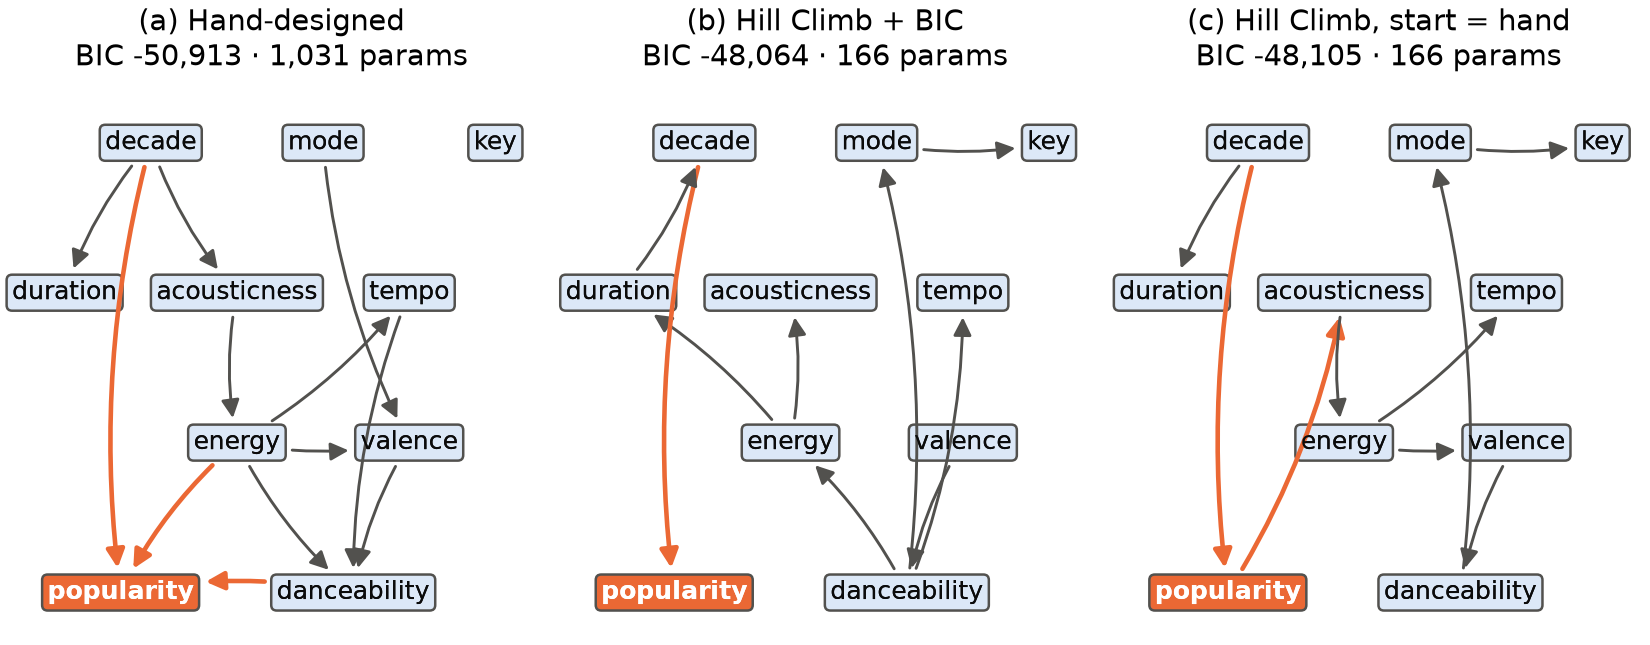
\includegraphics[width=\linewidth]{figures/structure/report_dags.png}
  \caption{(a) Hand-designed DAG. (b) Learned by HC + BIC from an empty graph. (c) HC + BIC started from (a), which has the lowest CV log-loss. Edges touching popularity are shown in orange.}
  \label{fig:dags}
\end{figure}

\begin{table}[t]
  \centering
  \caption{Structures compared on training-set BIC and 5-fold CV prediction of popularity from the other nine variables (add-one smoothed CPTs). HC = Hill Climb. Always predicting the majority class gives a CV accuracy of $0.332$.}
  \label{tab:structures}
  \small
  \setlength{\tabcolsep}{4pt}
\begin{tabular}{lrrrcc}
\toprule
Structure & Edges & Params & Train BIC & CV log-loss $\downarrow$ & CV acc.\ $\uparrow$ \\
\midrule
Hand-designed (proposal) & 12 & $1{,}031$ & $-50{,}913$ & 1.321 & 0.459 \\
\midrule
HC + BIC & 9 & $166$ & $-48{,}064$ & 1.312 & 0.463 \\
HC + BIC, start = hand & 9 & $166$ & $-48{,}105$ & \textbf{1.306} & 0.469 \\
GES (BIC) & 9 & $166$ & $-48{,}049$ & 1.311 & 0.466 \\
HC + AIC & 14 & $486$ & $-48{,}653$ & 1.312 & 0.468 \\
HC + BDeu (ESS 10) & 10 & $246$ & $-48{,}105$ & 1.311 & 0.466 \\
HC + K2 & 19 & $6{,}000{,}286$ & $\approx -24.6\,\mathrm{M}$ & 1.308 & 0.467 \\
PC ($\chi^2$, $\alpha{=}0.01$) & 9 & $590$ & $-50{,}098$ & 1.332 & 0.455 \\
Chow-Liu tree & 9 & $206$ & $-48{,}199$ & 1.311 & 0.466 \\
TAN & 17 & $934$ & $-50{,}511$ & 1.376 & 0.444 \\
Naive Bayes & 9 & $199$ & $-50{,}898$ & 1.380 & 0.454 \\
\midrule
Hand, decade $\to$ pop.\ only & 10 & $551$ & $-49{,}335$ & 1.331 & 0.463 \\
Empty graph (prior only) & 0 & $43$ & $-51{,}079$ & 1.402 & 0.332 \\
\bottomrule
\end{tabular}

\end{table}

\paragraph{Results.}
HC + BIC learns a sparse 166-parameter graph whose BIC ($-48{,}064$) far exceeds the hand DAG's ($-50{,}913$, 1{,}031 parameters; Table~\ref{tab:structures}). Most of the gap is popularity's CPT: an exhaustive search shows that a \emph{single} parent, decade, maximizes BIC. Compared up to Markov equivalence, the data confirms several of our feature edges: acousticness--energy, valence--danceability, energy--danceability and decade--duration each appear in at least $90\%$ of bootstrap runs. But all four v-structures in the hand DAG are rejected, and the proposed energy $\to$ valence edge appears in only $24\%$ of runs.

For prediction, the structures that link popularity to both decade and acousticness (HC started from the hand DAG, GES, Chow-Liu, AIC and BDeu) beat a decade-only model on all 5 folds (paired $\Delta$ log-loss $-0.020$ to $-0.025$). They reach about $47\%$ accuracy, against $33\%$ for the majority class. Naive Bayes and TAN do worse than decade-only on every fold. Fixing popularity's parents directly shows that decade + energy does as well as decade + acousticness (both better on 5/5 folds). Using both together overfits, and neither danceability nor duration is significant. In short, release decade dominates, and beyond it there is one small signal that the strongly correlated acousticness and energy carry interchangeably. We carry forward HC + BIC as the main model, Fig.~\ref{fig:dags}c for feature queries, and the hand DAG as a baseline.
